%TC第29.1节练习 4、5
%TC第29.2节练习 2、4、6
%TC第29.3节练习 5
%TC第29.4节练习 2
%%%%%%%%%%%%%%%%%%%%%%%%%%%%%%%%%%%%%%%%%%%%%%%%%%%%%%%%%%%%%%%%
\documentclass[11pt, a4paper, UTF8]{ctexart}
%%%%%%%%%%%%%%%%%%%%%%%%%%%%%%%%%%%
% File: preamble.tex
%%%%%%%%%%%%%%%%%%%%%%%%%%%%%%%%%%%

\usepackage[top = 1.5cm]{geometry}

% Set fonts commands
\newcommand{\song}{\CJKfamily{song}} 
\newcommand{\hei}{\CJKfamily{hei}} 
\newcommand{\kai}{\CJKfamily{kai}} 
\newcommand{\fs}{\CJKfamily{fs}}

\newcommand{\me}[2]{\author{{\bfseries 姓名:}\underline{#1}\hspace{2em}{\bfseries 学号:}\underline{#2}}}

% Always keep this.
\newcommand{\noplagiarism}{
  \begin{center}
    \fbox{\begin{tabular}{@{}c@{}}
      请独立完成作业,不得抄袭。\\
      若得到他人帮助, 请致谢。\\
      若参考了其它资料,请给出引用。\\
      鼓励讨论,但需独立书写解题过程。
    \end{tabular}}
  \end{center}
}

% Each hw consists of three parts:
% (1) this homework
\newcommand{\beginthishw}{\part{作业}}
% (2) corrections (Optional)
\newcommand{\begincorrection}{\part{订正}}
% (3) any feedback (Optional)
\newcommand{\beginfb}{\part{反馈}}

% For math
\usepackage{amsmath}
\usepackage{amsfonts}
\usepackage{amssymb}

% Define theorem-like environments
\usepackage[amsmath, thmmarks]{ntheorem}

\theoremstyle{break}
\theorembodyfont{\song}
\theoremseparator{}
\newtheorem*{problem}{题目}


\theoremheaderfont{\kai\bfseries}
\theoremseparator{:}
% \newtheorem*{remark}{注}
\theorempostwork{\bigskip\hrule}
\newtheorem*{solution}{解答}
\theorempostwork{\bigskip\hrule}
\newtheorem*{revision}{订正}

\theoremstyle{plain}
\newtheorem*{cause}{错因分析}
\newtheorem*{remark}{注}

\theoremstyle{break}
\theorempostwork{\bigskip\hrule}
\theoremsymbol{\ensuremath{\Box}}
\newtheorem*{proof}{证明}

\renewcommand\figurename{图}
\renewcommand\tablename{表}

% For figures
% for fig with caption: #1: width/size; #2: fig file; #3: fig caption
\newcommand{\fig}[3]{
  \begin{figure}[htp]
    \centering
      \includegraphics[#1]{#2}
      \caption{#3}
  \end{figure}
}

% for fig without caption: #1: width/size; #2: fig file
\newcommand{\fignocaption}[2]{
  \begin{figure}[htp]
    \centering
    \includegraphics[#1]{#2}
  \end{figure}
}
\usepackage{float}
\usepackage{indentfirst}
\usepackage{amsmath}
\usepackage{graphicx}
\usepackage{listings}
\usepackage{xcolor}
\usepackage{float}
\usepackage{enumerate}
\lstset{
	numbers=left,
	numberstyle= \tiny,
	keywordstyle= \color{ blue!70},
	commentstyle= \color{red!50!green!50!blue!50},
	rulesepcolor= \color{ red!20!green!20!blue!20} ,
	escapeinside=``, % 英文分号中可写入中文
	xleftmargin=2em,xrightmargin=2em, aboveskip=1em,
	framexleftmargin=2em
}
\title{机器学习导论}
\me{殷天润}{171240565}
\date{\today}

\begin{document}
\maketitle
\noplagiarism

%%%%%%%%%%%%%%%%%%%%%%%%%%%%%%%%%%%%%%%%%%%%%%%%%%%%%%%%%%%%%%%%
%                       Homework START!                        %
%%%%%%%%%%%%%%%%%%%%%%%%%%%%%%%%%%%%%%%%%%%%%%%%%%%%%%%%%%%%%%%%
\beginthishw
%%%%%%%%%%%%%%%%%%%%
\begin{problem}[ML problem 1]
Decision Tree I


 (1) [5pts] Assume there is a space contains three binary features $X$, $Y$, $Z$ and the objective function is $f(x,y,z)=\neg(x \text{ XOR } y)$. Let $H$ denotes the decision tree constructed by these three features. Please answer the following question: Is function $f$ realizable? If the answer is yes, please draw the decision tree $H$ otherwise please give the reason.\\
(2) [10pts] Now we have a dataset show by Table.1:\\
\begin{center}
	Table 1:example dataset\\
	\begin{tabular}{ccc|c}
		\hline
		$X$ & $Y$ & $Z$ & $f$\\
		\hline
		1 & 0 & 1 & 1\\
		1 & 1 & 0 & 0\\
		0 & 0 & 0 & 0\\
		0 & 1 & 1 & 1\\
		1 & 0 & 1 & 1\\
		0 & 0 & 1 & 0\\
		0 & 1 & 1 & 1\\
		1 & 1 & 1 & 0\\
		\hline
	\end{tabular}
\end{center}
Please use Gini value as partition criterion to draw the decision tree from the dataset. When Gini value is same for two features, please follow the alphabetical order.\\



\end{problem}
\begin{solution}
	\begin{enumerate}
		\item  Yes. It is realizable. The decision is as following:
		
		 \begin{figure}[htbp] 
			\centering
			\includegraphics[width=0.5\textwidth]{pro1_1.png}
			\caption{(Desicion tree of Pro 1.1)}
		\end{figure} 
	\item 选根节点:
	\begin{enumerate}
		\item Gini\_index(Z)=$\frac{2}{8}*(1-1)+\frac{6}{8}*(1-(\frac{4}{6})^2-(\frac{2}{6})^2)=\frac{1}{3}$
		\item 
		Gini\_index(Y)=$\frac{1}{2}*(1-0.5^2-0.5^2)*2$=0.5
		\item Gini\_index(X)=$\frac{1}{2}*(1-0.5^2-0.5^2)*2$=0.5
	\end{enumerate}
因此根节点为Z;

Z=0时,所有的f值都是0不用继续分类;

Z=1时,
\begin{enumerate}
	\item 	Gini\_index(Y)=$\frac{1}{2}*(1-(\frac{2}{3})^2-(\frac{1}{3})^2)*2$=0.44444
		\item 	Gini\_index(X)=$\frac{1}{2}*(1-(\frac{2}{3})^2-(\frac{1}{3})^2)*2$=0.44444
\end{enumerate}
根据字典序以X作为节点;

然后仅剩下Y作为其余结点;

决策树如图:
		 \begin{figure}[htbp] 
	\centering
	\includegraphics[width=0.5\textwidth]{pro1_2.png}
	\caption{(Desicion tree of Pro 1.2)}
\end{figure} 


	\end{enumerate}

    
\end{solution}




\begin{problem}[ML problem 2]
[25pts] {Decision Tree}

	Consider the following matrix:
$$
\left[
\begin{matrix}
24 & 53 & 23 & 25 & 32 & 52 & 22 & 43 & 52 & 48 \\
40 & 52 & 25 & 77 & 48 & 110 & 38 & 44 & 27 & 65\\
\end{matrix}
\right]
$$
which contains 10 examples and each example contains two features $x_1$ and $x_2$. The corresponding label of these 10 examples as follows:
$$
\left[
\begin{matrix}
1 & 0 & 0 &1 & 1 & 1 & 1& 0 & 0 & 1
\end{matrix}
\right]
$$
In this problem, we want to build a decision tree to do the classification task.
(1) [5pts] Calculate the entropy of the root node.\\
(2) [10pts] Building your decision tree. What is your split rule  and the classification error?\\
(3) [10pts] A multivariate decision tree is a generalization of  univariate decision trees, where more than one attribute can be used in the decision for each split. That is, the split need not be orthogonal to a feature's axis.

Building a multivariate decision tree where each decision rule is a linear classifier that makes decisions based on the sign of $\alpha x_1 + \beta x_2 - 1$. What is the depth of your tree, as well as $\alpha$ and $\beta$?

\end{problem}
\begin{solution}
\begin{enumerate}
	\item $-(p_1log_2~p_1+p_0log_2~p_0)=-(0.6*log_2~*0.6+0.4*log_2~*0.4)=0.9709505944546686$
	\item 我使用C程序计算了每一个以$x_1\geq x_{1i}$为划分,以及$x_2\geq x_{2i}$为划分的信息增益(Gain);
			 \begin{figure}[htbp] 
		\centering
		\includegraphics[width=0.5\textwidth]{gini1.png}
		\caption{(第一层信息增益($x_1\geq x_{1i}$))}
	\end{figure} 
	 \begin{figure}[htbp] 
	\centering
	\includegraphics[width=0.5\textwidth]{gini2.png}
	\caption{(第一层信息增益($x_2\geq x_{2i}$))}
\end{figure}
因此我选择$x_2\geq 38$作为划分;


因为$x_2<38$划分出来的两个元素label都是0,因此不需要继续划分;

现在考虑$x_2\geq 38$划分出来的8个元素,同理:
			 \begin{figure}[htbp] 
	\centering
	\includegraphics[width=0.5\textwidth]{gini21.png}
	\caption{(第二层信息增益($x_1\geq x_{1i}$))}
\end{figure} 
\begin{figure}[htbp] 
	\centering
	\includegraphics[width=0.5\textwidth]{gini22.png}
	\caption{(第二层信息增益($x_2\geq x_{2i}$))}
\end{figure}

因此选择$x_1\geq 43$作为划分;

此时,$x_1<43$的集合都是label为1的,不用继续划分;

仅仅需要划分$x_1\geq 43$的部分:
	 \begin{figure}[htbp] 
	\centering
	\includegraphics[width=0.5\textwidth]{gini31.png}
	\caption{(第三层信息增益($x_1\geq x_{1i}$))}
\end{figure} 
\begin{figure}[htbp] 
	\centering
	\includegraphics[width=0.5\textwidth]{gini32.png}
	\caption{(第三层信息增益($x_2\geq x_{2i}$))}
\end{figure}
此时根据上图划分$x_2\geq 65$,此时分出来的两类的label内部都一样,不必继续划分;

(Hint: C++代码见附件PRO2\_1.cpp,因为只是计算用途,所以基本没有可读性)

作决策树如下:

		 \begin{figure}[htbp] 
	\centering
	\includegraphics[width=0.5\textwidth]{pro2_1.png}
	\caption{(Desicion tree of Pro 2.2)}
\end{figure} 
\item 我调用了python的最小二乘法进行了计算,代码如图:
		 \begin{figure}[htbp] 
	\centering
	\includegraphics[width=1\textwidth]{code.png}
	\caption{(Code)}
\end{figure} 

结果是y=0.68196814-0.02264422*$x_1$+0.01454232*$x_2$;我调用了sklearn库的LineadRegression也得到了一样的结果;

代入进行预测,如果结果大于0.53label为1,小于0.5label为0,表格如下:

\begin{tabular}{|l|l|l|l|} %l(left)居左显示 r(right)居右显示 c居中显示
	\hline 
	$x_1$&$x_2$&label&0.68196814-0.02264422*$x_1$+0.01454232*$x_2$\\
	\hline  
	24&40&1&0.7201\\\hline 
	53&52&0&0.2380\\\hline 
	23&25&0&0.5247\\\hline 
	25&77&1&1.2356\\\hline 
	32&48&1&0.6553\\\hline 
	52&110&1&1.1041\\\hline 
	22&38&1&0.7364\\\hline 
	43&44&0&0.3481\\\hline 
	52&27&0&-0.1028\\\hline 
	48&65&1&0.5402\\
	\hline 
\end{tabular}

决策树如图:

	 \begin{figure}[htbp] 
	\centering
	\includegraphics[width=0.7\textwidth]{pro2_2.png}
	\caption{(Multivariate decision tree)}
\end{figure} 

\end{enumerate}

\end{solution}
\newpage
\begin{problem}[ML problem 3]
	[25pts] Convolutional Neural Networks


	\includegraphics[width=0.9\textwidth]{CNN.png}

	Using Fig. CNN as an example. Assuming that the loss function of the convolutional neural network is cross-entropy:
	
    \begin{enumerate}
	\item [(1)] [5 pts] Briefly describe the forward propagation process;
	\item [(2)] [5 pts] What is the difference between Relu and Sigmoid activation functions;
	\item [(3)] [5 pts] Derivation of the fully connected layer;
	\item [(4)] [5 pts] Derivation of the pooling layer with average pooling;
	\item [(5)] [5 pts] Derivation of the convolutional layer with Relu;
\end{enumerate}

	
\end{problem}

\begin{solution}
	\begin{enumerate}
		\item \begin{enumerate}
			\item 首先这是一个没有对原图像进行描边处理的卷积操作由$28\times 28$的输入变成了$6\times 24\times 24$(也就是深度为6)的卷积层$C_1$;
			\item 然后应该是经过了池化层进行了采样,从图片来看,kernel\_size应该是2,因此输入的是$6\times 24\times 24$输出的是$6\times 12\times 12$的$S_2$
			\item 然后再一次对$S_2$进行了卷积操作,输入是$6\times 12\times 12$的$S_2$,输出是$12\times 8\times 8$的$C_3$,由原先的6层深度变成了现在的12层深度
			\item 相似地,进行了池化层采样,kernel\_size应该也是2,变成了$12\times 4 \times  4$;
			\item 最后应该是经过了全连接层得到了最后的$12\times 1\times 1$的输出
			
		\end{enumerate}
	\item 	 \begin{figure}[htbp] 
		\centering
		\includegraphics[width=0.7\textwidth]{sigmod.png}
		\caption{Sigmod}
	\end{figure} 
\begin{figure}[htbp] 
	\centering
	\includegraphics[width=0.7\textwidth]{relu.png}
	\caption{Relu}
\end{figure} 
	\begin{enumerate}
		\item Sigmod函数和Relu函数都是激活函数;下面是不同点:
		\item Sigmod函数历史比较悠久,,把数压缩到0-1的连续函数之中,但是也有一些缺点,简而言之是Sigmod函数容易饱和,当输入非常大或者非常小的时候,神经元的梯度就接近于0了,并且输出不是0均值的,并且Sigmod函数的计算量会比Relu函数大一点;
		\item Relu函数是一个最近比较受欢迎的激活函数,Krizhevsky et al. 发现使用 ReLU 得到的SGD的收敛速度会比 sigmoid/tanh 快很多(如上图右)。有人说这是因为它是linear,而且梯度不会饱和
		;并且只要计算一个阈值,计算量小;
		
		但是Relu函数也有缺点,它在<0的时候都是0,容易神经元“坏死”,因为负梯度之后它永远都是0了;
	\end{enumerate}


\item 假设有损失函数$L:R^T\rightarrow R$,以及y=Wx+b;
根据链式法则:$\frac{\partial L}{\partial w}=DL(y(W))*Dy(W)$
由$y_1=\sum _j=1^{N}W_{1j}x_j+b1$

最后可以算到$\frac{\partial L}{\partial W}=\frac{\partial L}{\partial y}*x$
\item 池化层:
\begin{equation}
\begin{aligned}
\frac{\partial J(W,b;x,y)}{\partial b^{(l+1)}}&=\sum _{i=0}^{\frac{m-n+1}{r}-1}\sum^{\frac{m-n+1}{r}-1}_{j=0}\frac{\partial J(W,b;x,y)}{\partial z_{i,j}^{(l+1)}}\frac{\partial z_{i,j}^{l+1}}{\partial b^{(l+1)}}\\&=\sum _{i=0}^{\frac{m-n+1}{r}-1}\sum^{\frac{m-n+1}{r}-1}_{j=0}\delta _{i,j}^{l+1}
\end{aligned}
\end{equation}
\begin{equation}
\begin{aligned}
\frac{\partial J(W,b;x,y)}{\partial \beta^{(l+1)}}&=\sum _{i=0}^{\frac{m-n+1}{r}-1}\sum^{\frac{m-n+1}{r}-1}_{j=0}\frac{\partial J(W,b;x,y)}{\partial z_{i,j}^{(l+1)}}\frac{\partial z_{i,j}^{l+1}}{\partial \beta ^{(l+1)}}\\&=\sum _{i=0}^{\frac{m-n+1}{r}-1}\sum^{\frac{m-n+1}{r}-1}_{j=0}\delta _{i,j}^{l+1}\sum ^{(i+1)r-1}_{u=ir}\sum^{(j+1)r-1}_{v=jr}a_{u,v}^{(l)}
\end{aligned}
\end{equation}
\item 卷积层:
\begin{equation}
\begin{aligned}
\frac{\partial J(W,b;x,y)}{\partial b^{(l)}}&=\sum _{u=0}^{m-n} \sum _{v=0}^{m-n}\frac{\partial J(W,b;x,y)}{\partial z_{u,v}^{(l)}}\frac{z_{u,v}^{(l)}}{\partial b^{(l)}}\\&=\sum _{u=0}^{m-n} \sum _{v=0}^{m-n}\delta _{u,v}^{(l)}
\end{aligned}
\end{equation}
\begin{equation}
\begin{aligned}
\frac{\partial J(W,b;x,y)}{\partial k_{rot_{g,h}}^{(l)}}&=\sum _{u=0}^{m-n} \sum _{v=0}^{m-n}\frac{\partial J(W,b;x,y)}{\partial z_{u,v}^{(l)}}\frac{\partial z_{u,v}^{(l)}}{\partial _{g,h}^{(l)}}\\&=\sum _{u=0}^{m-n} \sum _{v=0}^{m-n}x_{rot_{u+g,v+h}}^{l-1}*\delta_{u,v}^{(l)}
\end{aligned}
\end{equation}
	\end{enumerate}
\end{solution}
\begin{remark}
	第二题参考了:$https://blog.csdn.net/yangdashi888/article/details/78015448$\\
	第三题参考了:$https://zhuanlan.zhihu.com/p/32836341$
	
	
\end{remark}

\begin{problem}[ML problem 4]
	In this task, you are asked to build a Convolutional Neural Networks (CNNs) from scratch and examine performance of the network you just build on \textbf{MNIST} dataset.

Fortunately, there are some out-of-the-box deep learning tools that can help you get started very quickly. For this task, we would like to ask you to work with the \textbf{Pytorch} deep learning framework. Additionally, Pytorch comes with a built-in dataset class for MNIST digit classification task in the \textbf{torchvision} package, including a training set and a validation set. You may find a pytorch introduction at 


${https://pytorch.org/tutorials/beginner/blitz/cifar10_tutorial.html}{here}$. Note that, you can use CPU or GPU for training at your choice.

Please find the detailed requirements below.

\begin{enumerate}
	\item[(1)] [5 pts] You are encouraged to implement the code using \emph{Python3}, implementations in any other programming language will not be judged. Please name the source file (which contains the main function) as \emph{CNN\underline{\hspace{0.5em}}main.py}. Finally, your code needs to print the performance on the provided validation set once executed.
	
	\item[(2)] [10 pts] Use any type of CNNs as you want and draw graphs to show your network architecture in the submitted report. You are encouraged to try more architectures.
	
	\item [(3)] [15 pts] During training, you may want to try some different optimization algorithms, such as SGD, Adam. Also, you need to study the effect of learning rate and the number of epoch, on the performance (accuracy).
	
	\item [(4)] [5 pts] Plot graphs (learning curves) to demonstrate the change of training loss as well as the validation loss during training.
\end{enumerate}
\end{problem}
\begin{solution}
   \begin{enumerate}
   	\item 我主要参考了Pytorch以及莫烦Python教程完成了我的代码,我的代码每50次就会输出一下目前的train\_loss,validation\_loss,最后会绘制四张图片:Train loss and validation loss,Epoch and validation loss,Epoch and accuracy,Training count and accuracy;然后输出最后的accuracy以及其他一些参数;
   	\item 一开始我参考了莫烦python构建了卷积$-->$relu激活$-->$池化$-->$卷积$-->$relu激活$-->$池化$-->$输出的网络,
   	\begin{figure}[htbp] 
   		\centering
   		\includegraphics[width=0.7\textwidth]{net1.png}
   		\caption{Net1}
   	\end{figure} 
   在 输入EPOCH=15,LR=0.0005,使用Adam方法学习的情况下:结果如下面的图片:
      	\begin{figure}[htbp] 
   	\centering
   	\includegraphics[width=0.7\textwidth]{result11.png}
   	\caption{Epoch and accuracy}
   \end{figure} 
   	\begin{figure}[htbp] 
	\centering
	\includegraphics[width=0.7\textwidth]{result12.png}
	\caption{Epoch and validation loss}
\end{figure} 
   
   	\begin{figure}[htbp] 
   	\centering
   	\includegraphics[width=0.7\textwidth]{result1.png}
   	\caption{Train loss and validation loss}
   \end{figure} 
   
  \newpage 
  然后我结合官网的教程做了一些改进,最后加了三层全连接并且倒数两个用Relu函数做了激活:
  此时网络是:卷积$-->$relu激活$-->$池化$-->$卷积$-->$relu激活$-->$池化$-->$全连接$-->$relu激活$-->$全连接$-->$relu激活$-->$输出的网络
      	\begin{figure}[htbp] 
   	\centering
   	\includegraphics[width=1.0\textwidth]{net2.png}
   	\caption{Net2}
   \end{figure} 

结果如下面的图片:
 	\begin{figure}[htbp] 
	\centering
	\includegraphics[width=0.7\textwidth]{result21.png}
	\caption{Epoch and accuracy}
\end{figure} 
\begin{figure}[htbp] 
	\centering
	\includegraphics[width=0.7\textwidth]{result22.png}
	\caption{Epoch and validation loss}
\end{figure} 

\begin{figure}[htbp] 
	\centering
	\includegraphics[width=0.7\textwidth]{result2.png}
	\caption{Train loss and validation loss}
\end{figure} 
\newpage

\item 我也探索了SGD,相对于Adam方法,SGD要求的学习率要更高一点,我在下图中是设置的0.01
   	\begin{figure}[htbp] 
	\centering
	\includegraphics[width=0.5\textwidth]{SGD.png}
	\caption{Training count and accuracy of SGD}
\end{figure} 
\newpage

对于adam方法,epoh与accuracy的关系我在第二问的图片中有放出,下面的图片是学习率与accuracy的关系,在这些数据中,我控制了Epoch为6:
   	\begin{figure}[htbp] 
	\centering
	\includegraphics[width=0.5\textwidth]{learning.png}
	\caption{学习率与accuracy的关系}
\end{figure} 
\item 这一问的图片上面几问都有相应的放出,总结下来一般情况下train\_loss的抖动会更大一点,并且如果过拟合比较严重的话,validation\_loss会比train\_loss高很多;
   \end{enumerate}
\end{solution}





%\begin{problem}[ML problem 5]

	%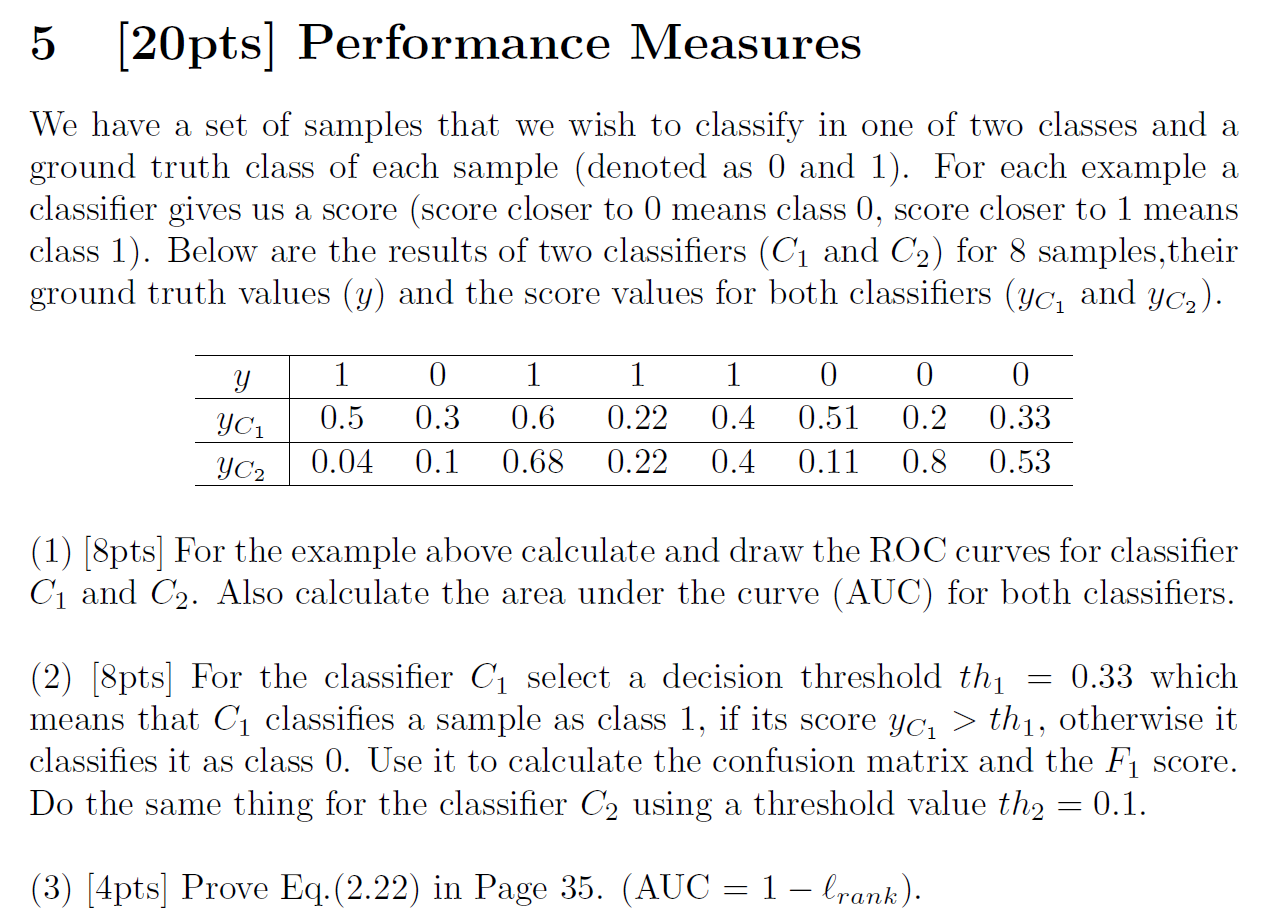
\includegraphics[scale=0.3]{5-p.png}

%\end{problem}
%\newpage
%\begin{solution}
   
%\end{solution}





%\begin{problem}[ML problem 6]
	
%\end{problem}
%\begin{solution}
    
%\end{solution}
%%%%%%%%%%%%%%%%%%%%%%%%%%%%%%%%%%%%%%%%%%%%%%%%%%%%%%%%%%%%%%%%
%                      Correction START!                       %
%%%%%%%%%%%%%%%%%%%%%%%%%%%%%%%%%%%%%%%%%%%%%%%%%%%%%%%%%%%%%%%%
%\begincorrection
%%%%%%%%%%%%%%%%%%%%
%\begin{problem}[]

%\end{problem}

%\begin{cause}
%
%\end{cause}

%\begin{revision}

%\end{revision}
%%%%%%%%%%%%%%%%%%%%
%\newpage
%%%%%%%%%%%%%%%%%%%%





%%%%%%%%%%%%%%%%%%%%%%%%%%%%%%%%%%%%%%%%%%%%%%%%%%%%%%%%%%%%%%%%
%                       Feedback START!                        %
%%%%%%%%%%%%%%%%%%%%%%%%%%%%%%%%%%%%%%%%%%%%%%%%%%%%%%%%%%%%%%%%
%\beginfb
%\begin{itemize}
%
%\end{itemize}





%%%%%%%%%%%%%%%%%%%%%%%%%%%%%%%%%%%%%%%%%%%%%%%%%%%%%%%%%%%%%%%%
%                        Homework END!                         %
%%%%%%%%%%%%%%%%%%%%%%%%%%%%%%%%%%%%%%%%%%%%%%%%%%%%%%%%%%%%%%%%
\end{document}
